\documentclass[a4paper, 12pt]{article}
\usepackage[english]{babel}
\usepackage[utf8]{inputenc}
\usepackage[T1]{fontenc}
\usepackage{lmodern}
\usepackage{hyperref}
\usepackage[numbers, sort&compress]{natbib}
\usepackage{calc}
\usepackage{nowidow}
\usepackage{color}
\usepackage{subcaption}
\usepackage{epsfig}
\usepackage{epstopdf}
\usepackage{verbatim}
\usepackage{enumitem}
\usepackage{graphicx}
\usepackage{amsfonts,amssymb,amsbsy} 
\usepackage{amsmath}
\usepackage{mathtools}
\usepackage{float}


\usepackage{pgfplots}
\usepackage{pgfplotstable}
\usepgfplotslibrary{units}
\usepgfplotslibrary{smithchart}
\pgfplotsset{compat=1.3,
	tick label style={font=\small},
	label style={font=\small},
	legend style={font=\footnotesize}}


\newlength{\oneLine}
\setlength{\oneLine}{12pt}

\newlength{\eqMargin}
\newlength{\eqHorizMargin}
\newlength{\eqVertMargin}

\setlength{\eqMargin}{20mm}
\setlength{\eqHorizMargin}{\eqMargin}
\setlength{\eqVertMargin}{\eqMargin}

% Paper
\setlength{\paperwidth}{210mm}
\setlength{\paperheight}{297mm}

% Rid the extra space
\setlength{\hoffset}{-1in}
\setlength{\voffset}{-1in}
\addtolength{\hoffset}{\eqHorizMargin}
\addtolength{\voffset}{\eqVertMargin}

% Set margin from the page border (horizontal)
\setlength{\oddsidemargin}{0pt}
\setlength{\evensidemargin}{0pt}

% Header
\setlength{\topmargin}{0pt}
\setlength{\headheight}{0pt}
\setlength{\headsep}{18pt}
%\renewcommand{\headrulewidth}{0pt}

% Footer
\addtolength{\footskip}{18pt}
%\renewcommand{\footrulewidth}{0pt}

% Margin notes
\setlength{\marginparsep}{0pt}
\setlength{\marginparwidth}{0pt}

% Text
\setlength{\textwidth}{\paperwidth - \hoffset - \hoffset - 25.4mm - 25.4mm}
\setlength{\textheight}{\paperheight - \voffset - \topmargin - \headheight - \headsep - \footskip - \voffset - 25.4mm - 25.4mm}

%\setlength{\labelwidth}{20mm}

% Hyperref settings
\hypersetup{
    unicode=true,					% non-Latin characters in Acrobat's bookmarks
    pdftoolbar=true,				% show Acrobat's toolbar?
    pdfmenubar=true,				% show Acrobat's menu?
    pdffitwindow=false,				% window fit to page when opened
    pdfstartview={FitH},			% fits the width of the page to the window
    pdftitle={S-26.3120 Radio Engineering, laboratory course},	% title
    pdfauthor={Tuomas Leinonen} {Gaurav Khairkar} {Lasse Toivanen},	% author
    pdfsubject={Radio Engineering},	% subject of the document
    pdfcreator={LaTeX},				% creator of the document
    pdfproducer={Aalto},			% producer of the document
    pdfkeywords={radio} {amplifier} {measurement},	% list of keywords
    pdfnewwindow=true,				% links in new window
    colorlinks=true,				% false: boxed links; true: colored links
    linkcolor=black,				% color of internal links
    citecolor=black,				% color of links to bibliography
    filecolor=black,				% color of file links
    urlcolor=black					% color of external links
}

% Bad hyphenation
%\hyphenation{}

\newcommand{\dB}{\ensuremath{\mathrm{dB}}}

\definecolor{dkred}{rgb}{0.6, 0, 0}
\definecolor{dkgrn}{rgb}{0, 0.6, 0}
\definecolor{dkblue}{rgb}{0, 0, 0.6}

\newcommand*{\mysection}[1]{%
\newpage%
\section*{#1}%
\addcontentsline{toc}{section}{#1}%
}

\pagestyle{plain}


\begin{document}

\begin{titlepage}
\pagestyle{empty}
\begin{center}

\vspace*{30mm}
\noindent\LARGE{\textbf{S-26.3120 Radio Engineering, laboratory course}}

\vspace*{20mm}

\Large{\textbf{Lab 4: Amplifier}}\\

\vspace*{15mm}

\large{\textbf{Final Report}}\\
\vspace{15mm}
\large{\today}
	
\vspace*{30mm}
\large{
	\begin{tabular}{l l}
		\textbf{Group 1:} 				& \\
		Tuomas Leinonen 				& 84695P \\
		Gaurav Khairkar					& 12345A \\
		Lasse Toivanen					& 12345A
	\end{tabular}
}

\end{center}

\end{titlepage}

\mysection{Abstract}

Text

\newpage
\addcontentsline{toc}{section}{Contents}
\tableofcontents

\mysection{Symbols and abbreviations}

\subsection*{Symbols}

	\begin{description}[font=\rmfamily\mdseries, leftmargin=25.5mm, style=sameline, align=right, labelsep=5mm, itemsep=-2pt]
		\item[$R$]					resistance [$\Omega$]
		\item[$C$]					capacitance [F]
		\item[$L$]					inductance [H]
		\item[$f$] 					frequnecy [Hz]
		\item[$Z$] 					impedance [$\Omega$]
		\item[$Y$] 					admittance [S]
		\item[$z$] 					normalized impedance
		\item[$y$] 					normalized admittance
		\item[$\lambda$] 			wavelength [m]
		\item[$F$] 					noise figure [dB]
		\item[$G$] 					two-port gain equal to $|S_{21}|$ [dB]
		\item[$L$] 					attenuation [dB]
		\item[$S_{ij}$] 			scattering parameter from port $i$ to port $j$
		\item[$\mathit{BW}$] 		bandwidth [Hz]
		\item[$\mathit{IIP}_n$] 	$n$th order input-referred intermodulation intercept point [dBm]
		\item[$\mathit{IM}_n$] 		$n$th order intermodulation product [dBm]
		\item[$\mathit{ICP}$] 		1~dB input compression point [dBm]
		\item[$P$] 					signal power [dBm]
		\item[$N$] 					noise power [dBm]
		\item[$T$] 					temperature [K]
		\item[$w$] 					transmission line width [m]
		\item[$h$] 					substrate height [m]
		\item[$\tan \delta$]		``tangent delta'', a merit of substrate quality (attenuation)
		\item[$\epsilon_\mathrm{r}$]			relative permittivity of the substrate
		\item[$V$]					voltage [V]
		\item[$I$]					current [I]
		\item[$U$]					unilateral figure of merit [U]
		\item[$\Delta$]				determinant of a scattering matrix
		\item[$K$]					Rollet's stability factor
		\item[$\mu$]				stability factor
		\item[$\rho$]				reflection coefficient
		\item[$\textit{RL}$] 		return loss [dB]
		\item[$l$]					transmission line length
	\end{description}

\newpage
\subsection*{Abbreviations}

	\begin{description}[font=\rmfamily\mdseries, leftmargin=25.5mm, style=sameline, align=right, labelsep=5mm, itemsep=-2pt]
		\item[LNA]					low-noise amplifier
		\item[SMA]					SubMiniature version A, a type of coaxial connector
		\item[pHEMT]				pseudomophic high electron mobility transistor, a type of field-effect transistor
		\item[RF]					radio frequency
		\item[DC]					direct current
		\item[CS]					common source, a type of field-effect transistor configuration
		\item[IDCS]					inductively degenerated common source
		\item[PTH]					plated-through hole, a via
		\item[PCB]					printed circuit board
	\end{description}

\newpage
\section{Introduction}

Text

\newpage
\section{Theoretical background}

Text

\newpage
\section{Preliminary design}

\begin{figure}[!h]
	\begin{center}
		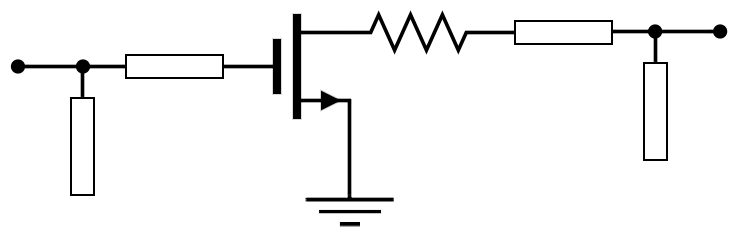
\includegraphics[scale=1]{img/pre.png}
		\setlength{\unitlength}{1mm}
		\begin{picture}(1,1)
			\put(-71, 13.3){\small IN}
			\put(-56.5, 16.7){\small$0.177\;\lambda$}
			\put(-72.5, 6){\small$0.136\;\lambda$}
			\put(-34, 12){\small$100\;\Omega$}
			\put(-23.5, 19.5){\small$0.306\;\lambda$}
			\put(-7, 9){\small$0.135\;\lambda$}
			\put(-1, 16){\small OUT}
		\end{picture}
		\caption{Amplifier pre-design ($Z_0 = 50\;\Omega$).}
		\label{f:c}
	\end{center}
\end{figure}

\newpage
\section{Design}

After obtaining a preliminary starting point for the design it was time to pursue 
the actual design with ADS simulations. In ADS, the final balancing resistor, 
biasing networks and matching networks were to be designed and optimized. For 
the simulations, the used PCB material was assigned as RT-Duroid 5870 (Cu 1.0 oz/ft$^2$) 
with $\epsilon_\mathrm{r} = 2.33 \pm 0.02$, $h = 0.787 \pm 0.003$~mm, $t = 35$~um, and $\tan \delta = 0.0012$. 
The dimensions of the circuit board were $70 \times 85 \; \mathrm{mm}^2$. Fig. \ref{f:lo} 
presents the final amplifier layout. The layout comprises of five individual 
sections, namely, the transistor section (a), input and output biasing networks 
(a,b) and input and output matching networks (d,e). 

\begin{figure}[!h]
	\begin{center}
		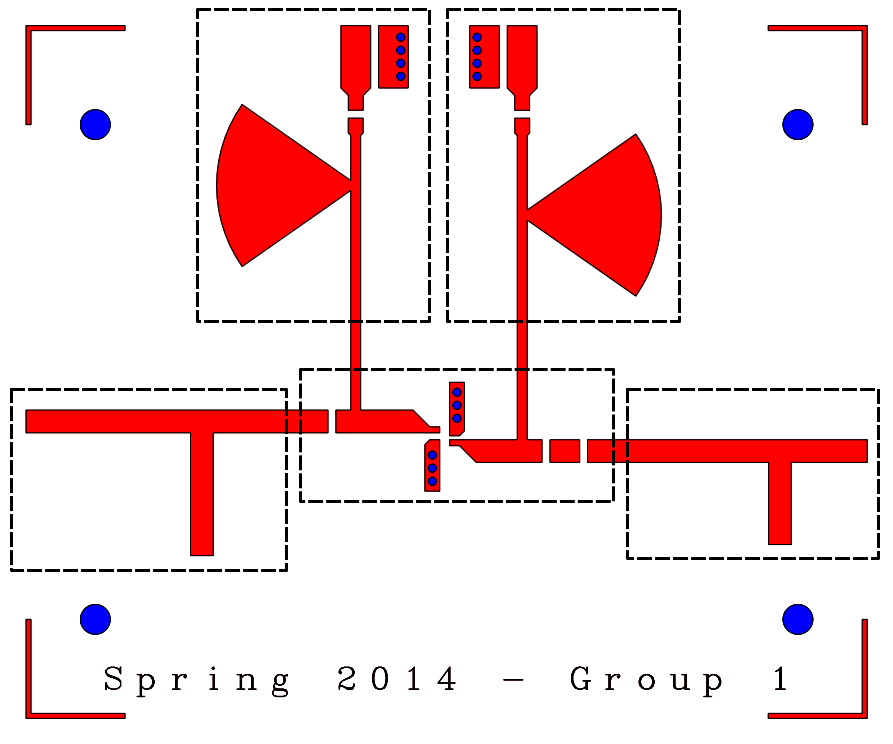
\includegraphics[scale=1]{img/layout.png}
		\setlength{\unitlength}{1mm}
		\begin{picture}(1,1)
			\put(-32, 27.5){\small{(a)}}
			\put(-60.5, 58){\small{(b)}}
			\put(-26.5, 58){\small{(c)}}
			\put(-76, 17){\small{(d)}}
			\put(-9.4, 18){\small{(e)}}
		\end{picture}
		\caption{The final amplifier layout comprising of: (a) Transistor section, (b) Input biasing, 
			(c) Output biasing, (d) Input matching and (e) Output matching.}
		\label{f:lo}
	\end{center}
\end{figure}



The transistor section includes the transistor followed by the stabilizing resistor. 
The two gaps at the input and output are for the DC blocking capacitors (10 pF, MURATA GQM series). 
The capacitors prevent the DC power from flowing to the input and output of the amplifier. 
The lines pointing vertically from the transistor are for the source. The three blue dots
on the source lines are the via-grounding holes. Using multiple via-holes lowers the inductance 
to the ground. An initial value for the balancing resistor was obtained from the preliminary 
design. The validity of the preliminary design was quickly checked with a S-parameter model 
of the transistor. The S-parameter model contains the S-parameters of a certainly biased 
transistor and thus does not require biasing networks. As the preliminary 100 $\Omega$ 
stabilizing resistor seemed valid it was time to replace the transistor with its non-linear 
model and continue with the design of the biasing networks. 

The biasing networks were designed separately and their operation was verified before attaching 
them to the actual amplifier model. The main purpose of a biasing networks is to provide DC 
voltage to empower the transistor. The DC power should not couple to the input and output of 
the amplifier nor should the RF signal flow to the DC source. Coupling can be avoided by, for 
instance, using DC blocks, radial stubs, signal absorbing resistors and shorting capacitors. 
A radial stub, placed at a distance of quarter wavelength from the original signal path, creates 
a virtual open circuit for the RF signal at a certain frequency. Thus the RF signal does not 
propagate to the DC source. The absorbing resistor and shorting capacitors are placed to account 
for the possible non-desired RF signals. The  resistor after the radial stub absorbs the possible 
reflections whereas the capacitors short the RF signals directly to the ground. 15 $\Omega$ 
absorbing resistors were found to be adequate. Three capacitors (1 pF, 10 pF and 100 pF, MURATA 
GQM series) were used for the shorting. Due to the non-ideality of the capacitors they provide 
an enhanced shorting to the ground. The grounding was made using four via-holes. The correct 
biasing gate to source voltage, $V_{\mathrm{GS}}$ was derived with an DC analysis in which the 
$V_{\mathrm{GS}}$ was swept to result in the required biasing current $I_{\mathrm{DS}}$. The 
result of the DC analysis is presented in Fig. \ref{Sim_Bias_point}. Thus the correct biasing 
was achieved with $V_{\mathrm{GS}}=-0.39 \,\mathrm{V}$. The voltage drop due to the absorbing 
resistor should be accounted by increasing the source DC voltage by the equivalent amount. In 
the input biasing network the voltage drop is insignificant due to the low current whereas at 
the output it is significant, namely, $15 \, \Omega * 30 \, \mathrm{mA} = 0.45 \,\mathrm{V}$.

\begin{figure}[!h]
\centering
\begin{tikzpicture}
\begin{axis}[
/pgf/number format/.cd,
1000 sep={},
ylabel=$I_\mathrm{DS} \, \mathrm{[mA]}$,
xlabel=$V_\mathrm{DS} \, \mathrm{[V]}$,
width=3.5in,
height=1.86in,
ymin=0,
ymax=45,
xmax=5,
xmin=0,
ytick={0,5,...,45},
grid=both,
%legend cell align=left,
%legend style={
%at={(0.01,0.02)},
%anchor=south west}
legend pos=south east
]
\addplot+[mark=none, color=red, solid] table[x=VDS,y=IDS_VGS_m44] {data/Simulations/Bias_point_all.txt};
\addlegendentry{$V_\mathrm{GS} = -4.4$~V}
\addplot+[mark=none, color=blue, solid] table[x=VDS,y=IDS_VGS_m39] {data/Simulations/Bias_point_all.txt};
\addlegendentry{$V_\mathrm{GS} = -3.9$~V}
\addplot+[mark=none, color=green, solid] table[x=VDS,y=IDS_VGS_m34] {data/Simulations/Bias_point_all.txt};
\addlegendentry{$V_\mathrm{GS} = -3.4$~V}
\addplot+[sharp plot, mark=none, color=black, solid] coordinates
{(2,-1) (2,50)};
\addplot+[sharp plot, mark=none, color=black, solid] coordinates
{(-1,30) (6,30)};
\end{axis}
\end{tikzpicture}
\caption{Bias point DC analysis. 
\label{Sim_Bias_point}}
\end{figure}

After designing the biasing networks they were attached to the amplifier. 
Correctly designed biasing networks should provide similar simulation results 
as the S-parameter model of the transistor.

The input and output matching was done using a single open stub. The lengths 
of the transmission lines were tuned carefully using the Smith chart to meet 
the design criteria on the amplifier center frequency. At this point, the 
amplifier did not meet the set gain criteria and thus the value of the balancing 
resistor had to be decreased. A suitable compromise was found with a balancing 
resistor value of 50~$\Omega$. 

Fig. \ref{f:sim} presents the final simulation results for the input 
and output return losses $RL$, stability factor $K$, gain $G$ and noise figure 
$F$. The simulation results depict the amplifier to satisfy all of the set design 
specifications. The final results at the design frequency of 2.5~GHz are: 
$\textit{RL}_\mathrm{in} = 22.5 \;\dB$, $\textit{RL}_\mathrm{out} = 29.5 \;\dB$, 
$K = 1.50$, $G = 13.86 \;\dB$ and $F = 0.53 \;\dB$.

\begin{figure}[!h]
\centering
%\begin{center}
\begin{tabular}{cc}
\begin{tikzpicture}[baseline,trim axis left]
\begin{axis}[
/pgf/number format/.cd,
1000 sep={},
ylabel=$S_{ii} \, \mathrm{[dB]}$,
xlabel=Frequency f $\mathrm{[GHz]}$,
width=3in,
height=1.86in,
ymin=-35,
ymax=5,
xmax=3.5,
xmin=1.5,
ytick={-35,-30,...,5},
grid=both,
%legend cell align=left,
%legend style={
%at={(0.01,0.02)},
%anchor=south west}
legend pos=south west
]
\addplot+[mark=none, color=red, solid] table[x=freq,y=S11] {data/Simulations/Simulation_results_all.txt};
\addlegendentry{$S_{11}$}
\addplot+[mark=none, color=blue, solid] table[x=freq,y=S22] {data/Simulations/Simulation_results_all.txt};
\addlegendentry{$S_{22}$}

\end{axis}
\end{tikzpicture}

&

\hspace{25pt}
\begin{tikzpicture}[baseline,trim axis left]
\begin{axis}[
/pgf/number format/.cd,
1000 sep={},
ylabel=Stability factor $\mu$,
xlabel=Frequency f $\mathrm{[GHz]}$,
width=3in,
height=1.86in,
ymin=0,
ymax=2.5,
xmax=3.5,
xmin=1.5,
ytick={0,0.5,...,2.5},
grid=both,
%legend cell align=left,
%legend style={
%at={(0.01,0.02)},
%anchor=south west}
%legend pos=south east
]
\addplot+[mark=none, color=red, solid] table[x=freq,y=Stability] {data/Simulations/Simulation_results_all.txt};

\end{axis}
\end{tikzpicture}
\\
%
\begin{tikzpicture}[baseline,trim axis left]
\begin{axis}[
/pgf/number format/.cd,
1000 sep={},
ylabel=Gain $G$ $\mathrm{[dB]}$,
xlabel=Frequency f $\mathrm{[GHz]}$,
width=3in,
height=1.86in,
ymin=0,
ymax=15,
xmax=3.5,
xmin=1.5,
ytick={0,3,...,15},
grid=both,
%legend cell align=left,
%legend style={
%at={(0.01,0.02)},
%anchor=south west}
%legend pos=south east
]
\addplot+[mark=none, color=red, solid] table[x=freq,y=Gain] {data/Simulations/Simulation_results_all.txt};

\end{axis}
\end{tikzpicture}

&

\hspace{25pt}
\begin{tikzpicture}[baseline,trim axis left]
\begin{axis}[
/pgf/number format/.cd,
1000 sep={},
ylabel=Noise figure $F$ $\mathrm{[dB]}$,
xlabel=Frequency f $\mathrm{[GHz]}$,
width=3in,
height=1.86in,
ymin=0,
ymax=6,
xmax=3.5,
xmin=1.5,
ytick={0,1,...,6},
grid=both,
%legend cell align=left,
%legend style={
%at={(0.01,0.02)},
%anchor=south west}
%legend pos=south east
]
\addplot+[mark=none, color=red, solid] table[x=freq,y=Noise] {data/Simulations/Simulation_results_all.txt};

\end{axis}
\end{tikzpicture}
\\
\end{tabular}
\caption{Simulation results for input and output return losses, stability factor, gain and noise.}
\label{f:sim}
\end{figure}

Fig. \ref{f:hb} illustrates the 1 dB gain compression and third order intercept 
(TOI) point for the amplifier. The second and third order intermodulation terms ($\textit{IM}_2$ and $\textit{IM}_3$) 
are also plotted in addition to the desired signal frequency. The 1-dB gain compression and TOI occur 
at input power levels of $-1.3$~dB and 6.7~dB, respectively. 

\begin{figure}[!h]
\centering
%\begin{tabular}{cc}
\begin{tikzpicture}%[baseline, trim axis left]
\begin{axis}[
/pgf/number format/.cd,
1000 sep={},
ylabel=Gain G $\mathrm{[dB]}$,
xlabel=$P_\mathrm{in} \; \mathrm{[dBm]}$,
width=6in,
height=4in,
ymin=0,
ymax=15,
xmax=15,
xmin=-30,
ytick={0,3,...,15},
grid=both,
%legend cell align=left,
%legend style={
%at={(0.01,0.02)},
%anchor=south west}
%legend pos=south east
]
\addplot+[mark=none, color=red, solid] table[x=P_in,y=Gain] {data/Simulations/Simulation_HB_results_all.txt};

\addplot [black, mark=*, mark options={draw=black}]
coordinates {
(-1.3,12.8589) 
};

\node at (axis cs:-1.3,12.8589) [anchor=south west] {1-dB compression};

\end{axis}
\end{tikzpicture}
%&
\begin{tikzpicture}[baseline]
\begin{axis}[
/pgf/number format/.cd,
1000 sep={},
ylabel=$V_\mathrm{out} \; \mathrm{[dBm]}$,
xlabel=$P_\mathrm{in} \; \mathrm{[dBm]}$,
width=6in,
height=4in,
ymin=-85,
ymax=35,
xmax=15,
xmin=-30,
ytick={-85,-65,...,35},
grid=both,
legend cell align=left,
%legend style={
%at={(0,1.02)},
%anchor=south west}
legend pos=south east
]
\addplot+[mark=none, color=red, solid] table[x=P_in,y=V_out] {data/Simulations/Simulation_HB_results_all.txt};
\addlegendentry{Fundamental}
\addplot+[mark=none, color=green, dashed] table[x=P_in,y=V_out_2H] {data/Simulations/Simulation_HB_results_all.txt};
\addlegendentry{$\mathit{IM}_2$}
\addplot+[mark=none, color=blue, densely dashed] table[x=P_in,y=V_out_3H] {data/Simulations/Simulation_HB_results_all.txt};
\addlegendentry{$\mathit{IM}_3$}

\addplot+[mark=none, color=red, densely dotted] table[
x=P_in,
y={create col/linear regression={y=V_out, 
%variance list is used to weight the selection of points. Dummy solution. Not good.
variance list={1,1,1,1,1,1,1,1,1,1,
1,1,1,1,1,1,1,1,1,1,
1,1,1,1,1,1000,
1000,1000,1000,1000,1000,1000,1000,1000,1000,1000,
1000,1000,1000,1000,1000,1000,1000,1000,1000,1000}
}}]
{data/Simulations/Simulation_HB_results_all.txt};

\addplot+[mark=none, color=blue, densely dotted] table[
x=P_in,
y={create col/linear regression={y=V_out_3H,
%variance list is used to weight the selection of points. Dummy solution. Not good. 
variance list={1000,1000,1000,1000,1000,1000,1000,1000,1000,1000,
1000,1000,1000,1000,1000,1000,1000,1000,1000,1000,
1000,1000,1000,1000,1000,1,1,1,1,1,1,1000,1000,1000,1000,1000,
1000,1000,1000,1000,1000,1000,1000,1000,1000,1000}
}}]
{data/Simulations/Simulation_HB_results_all.txt};

\addplot [black, mark=*, mark options={draw=black}]
coordinates {
(6.7,20.5) 
};

\node at (axis cs:6.7,20.5) [anchor=south east] {TOI};

\end{axis}
\end{tikzpicture}
%\\
%\end{tabular}

\caption{Simulation results for gain saturation and TOI.}
\label{f:hb}
\end{figure}

\newpage
\section{Measurements}

Text

\newpage
\section{Results}

Text

\newpage
\section{Conclusions}

Text

\newpage
\section{Feedback}

Text


\newpage
\begin{thebibliography}{9}%\itemsep 7pt\parskip -5pt 
	
\bibitem{lsh} C.\ Icheln (edited), 
	\textit{Lecture supplement handout},
	S-26.3120 Laboratory course in Radio Engineering course material.
	
\bibitem{bahl} I.\ J.\ Bahl, 
	\textit{Fundamentals of RF and Microwave Transistor Amplifiers},
	J.\ Wiley \& Sons, 2009.

\bibitem{gonz} G.\ Gonzalez, 
	\textit{Microwave Transistor Amplifiers -- Analysis and Design},
	Prentice Hall, 2nd Ed., 1997.
	
\bibitem{pozar} D.\ M.\ Pozar, 
	\textit{Microwave Engineering}, 
	J.\ Wiley \& Sons, 4th Ed., 2012.

\end{thebibliography}

\end{document}
